

\begin{figure}[tb]
  \begin{center}
    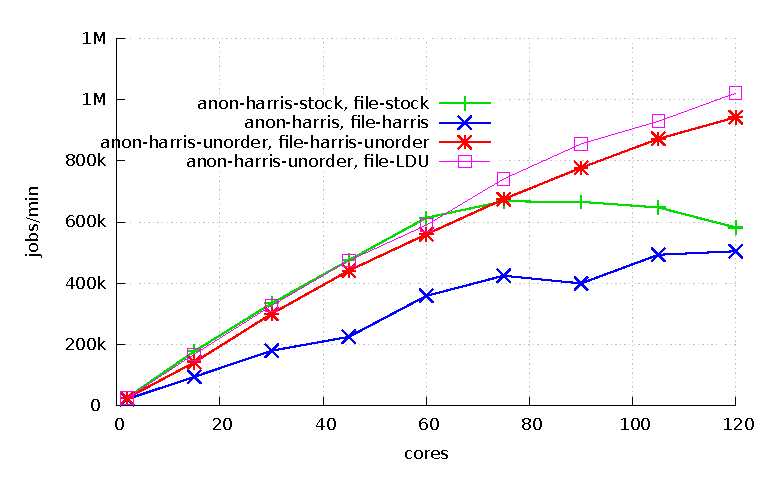
\includegraphics[scale=0.65]{graph/aim7.eps}
  \end{center}
  \caption{Scalability of AIM7 multiuser for different method.  The combination
  \deferu with unordered harris list scale well;in contrast, up to 60 core, the
  stock Linux scale linearly, then it  flattens out.}
  \label{fig:aim7}
\end{figure}

\section{Evaluation}



\begin{figure*}[tb]
    \centering
    \begin{subfigure}[b]{0.33\textwidth}
        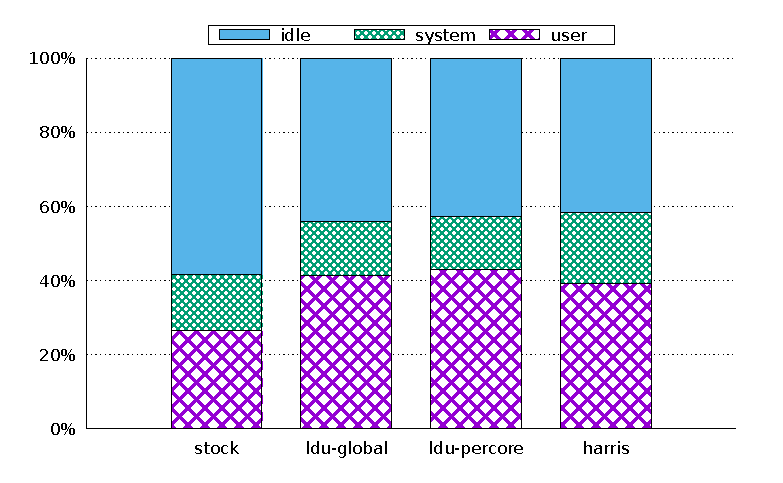
\includegraphics[height=1.3in]{graph/aim7_cpuutils.eps}
        \caption{AIM7 - 120core}
    \end{subfigure}%
    \begin{subfigure}[b]{0.33\textwidth}
        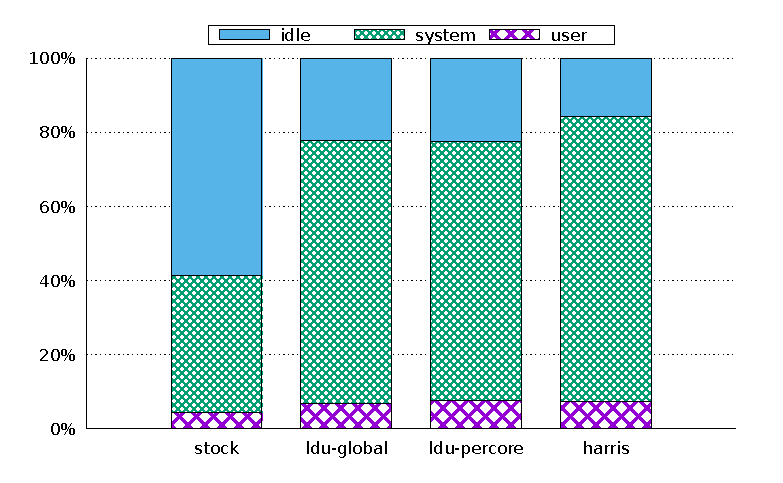
\includegraphics[height=1.3in]{graph/exim_cpuutils.eps}
        \caption{Exim - 120core}
    \end{subfigure}
    \begin{subfigure}[b]{0.33\textwidth}
        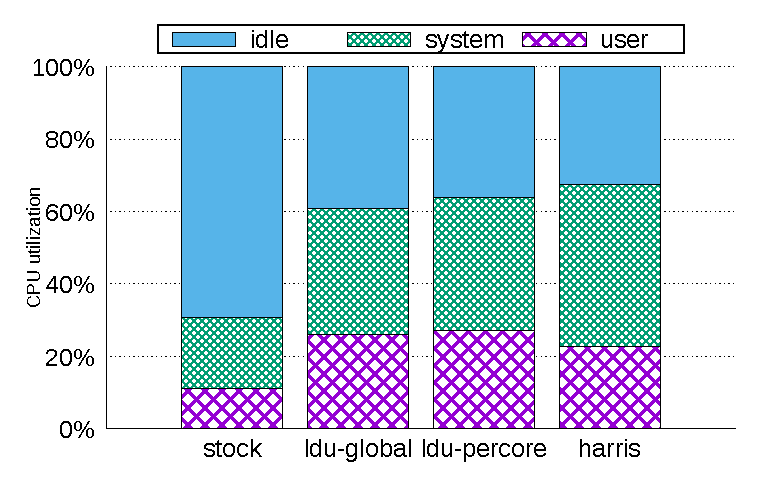
\includegraphics[height=1.3in]{graph/lmbench_cpuutils.eps}
        \caption{Lmbench - 120core}
    \end{subfigure}
        \centering
    \caption{Read-write ratio from 50:50 to 1:99 percent}
    \label{fig:utilization}
    
\end{figure*}


%$$$$$$$$$$$$$$$$$$$$$$$$$$$$$$$$$$$$$$$$$$$$$$$$$$$$$$$$$$$$$$$$$$$$$$$$$$$$$$$$
%Paragraph 1: 무엇을 평가 했는지에 대한 설명 
%$$$$$$$$$$$$$$$$$$$$$$$$$$$$$$$$$$$$$$$$$$$$$$$$$$$$$$$$$$$$$$$$$$$$$$$$$$$$$$$$

\subsection{Experimental setup}

%$$$$$$$$$$$$$$$$$$$$$$$$$$$$$$$$$$$$$$$$$$$$$$$$$$$$$$$$$$$$$$$$$$$$$$$$$$$$$$$$
%Paragraph 3: 운영체제 및 커널 버전 설명
%$$$$$$$$$$$$$$$$$$$$$$$$$$$$$$$$$$$$$$$$$$$$$$$$$$$$$$$$$$$$$$$$$$$$$$$$$$$$$$$$
We ran the three benchmarks on Linux 4.5.0-rc6 with stock Linux. 
All experiments were performed on a 120 core machine with 8-socket, 15-core
Intel E7-8870 chips equipped with 792 GB DDR3 DRAM.

%$$$$$$$$$$$$$$$$$$$$$$$$$$$$$$$$$$$$$$$$$$$$$$$$$$$$$$$$$$$$$$$$$$$$$$$$$$$$$$$$
%Paragraph 1: 벤치 마크 대한 설명
%$$$$$$$$$$$$$$$$$$$$$$$$$$$$$$$$$$$$$$$$$$$$$$$$$$$$$$$$$$$$$$$$$$$$$$$$$$$$$$$$
Fork-intensive applications benefit from the designs described in this
research, so we use well-known three fork-intensive benchmarks:AIM7, a Linux
scalability benchmark;Exim, an email server in MOSBENCH;and Lmbench, a micro
benchmark.
The workloads exhibit the high lock contentions because of the reverse mapping.
Moreover, the AIM7 benchmark is widely used in the Linux community not only for
testing the Linux kernel but also for improving the scalability. 
The Exim is a real world application, but it has scalability bottlenecks caused
by the Linux fork.
Finally, in order to only focus on the fork performance and scalability, we
selected the Lmbench.

%$$$$$$$$$$$$$$$$$$$$$$$$$$$$$$$$$$$$$$$$$$$$$$$$$$$$$$$$$$$$$$$$$$$$$$$$$$$$$$$$
%Paragraph 2-1: Harris Lock free list 구현 내용에 대한 설명 
%$$$$$$$$$$$$$$$$$$$$$$$$$$$$$$$$$$$$$$$$$$$$$$$$$$$$$$$$$$$$$$$$$$$$$$$$$$$$$$$$
To compare our \deferu implementation to a concurrent non-blocking
Harris linked list ~\cite{Harris2001Lockfree}, we additionally implemented the
Harris linked list to Linux kernel.
The Harris linked list refers from sysnchrobench~\cite{Gramoli2015Synchrobench}
and ASCYLIB~\cite{David2015ASYNCHRONIZED}, and we slightly convert the
Harris linked list to Linux kernel style.
In addition, we replace the two rmaps data structure to the Harris linked list.
Since the Harris linked list in the synchrobench and the ASCYLIB leaks memory,
we implemented a garbage collector for the Linux kernel using the Linux's work
queues and non-blocking linked list.

%$$$$$$$$$$$$$$$$$$$$$$$$$$$$$$$$$$$$$$$$$$$$$$$$$$$$$$$$$$$$$$$$$$$$$$$$$$$$$$$$
%Paragraph 2: 비교 대상에 대한 설명
%$$$$$$$$$$$$$$$$$$$$$$$$$$$$$$$$$$$$$$$$$$$$$$$$$$$$$$$$$$$$$$$$$$$$$$$$$$$$$$$$
We used four different experiment settings. 
First, we used the stock Linux as the baseline reference. 
Second, we used Harris lock-free list version of the Linux kernel as we
mentioned earlier.
Next, we used the LDU version of the Linux kernel that used global queue.
Finally, we used the per-core queue version of LDU in the Linux.
Unfortunately, since we could not obtain the detailed implementation of the
Oplog, we excluded the comparison of between \deferu and Oplog in this paper.

\subsection{AIM7}

%$$$$$$$$$$$$$$$$$$$$$$$$$$$$$$$$$$$$$$$$$$$$$$$$$$$$$$$$$$$$$$$$$$$$$$$$$$$$$$$$
%Paragraph 1: AIM7 실험 결과
%$$$$$$$$$$$$$$$$$$$$$$$$$$$$$$$$$$$$$$$$$$$$$$$$$$$$$$$$$$$$$$$$$$$$$$$$$$$$$$$$


%$$$$$$$$$$$$$$$$$$$$$$$$$$$$$$$$$$$$$$$$$$$$$$$$$$$$$$$$$$$$$$$$$$$$$$$$$$$$$$$$
%Paragraph 1: 워크로드에 대한 설명
%$$$$$$$$$$$$$$$$$$$$$$$$$$$$$$$$$$$$$$$$$$$$$$$$$$$$$$$$$$$$$$$$$$$$$$$$$$$$$$$$
We used AIM7-multiuser, which is one of fork-intensive workload in AIM7.
The multiuser workload simultaneously creates many processes with various
operations(section 2()), and we uses the temp filesystem to minimize the file
system bottleneck.
We increase the number of users for input.
 
%$$$$$$$$$$$$$$$$$$$$$$$$$$$$$$$$$$$$$$$$$$$$$$$$$$$$$$$$$$$$$$$$$$$$$$$$$$$$$$$$
%Paragraph 2: 실험 결과에 대한 설명
%$$$$$$$$$$$$$$$$$$$$$$$$$$$$$$$$$$$$$$$$$$$$$$$$$$$$$$$$$$$$$$$$$$$$$$$$$$$$$$$$
The results for AIM7-multiuser are shown in Figure~\ref{fig:aim7}, and the
results show the throughput of AIM7-multiuser with our four different settings.
Up to 75 core, the stock Linux scales linearly and then serialized updates
become bottlenecks.
However, up to 120core, Harris and our LDU scale well because
these workloads can concurrently execute update operations without the
reader-writer semaphores(\code{anonymous} and \code{file}).
The per-core queue version of LDU has the best performance and
scalability outperforming stock Linux by 1.5x and Harris by
1.1x.
Although the global queue version of LDU has the global CAS operation, it
also has high performance and scalability because the CAS operations are
mitigated by two LDU techniques, it has decreased 2\% performance compared with
per-core queue.
The stock Linux has the highest idle time(58\%) since it waits to acquire
semaphore(\code{anon\_vma's rwsem} and \code{file's i\_mmap\_rwsem}).
Surprisingly, although LDU has higher idle time than Harris, the throughput is
higher than Harris because LDU is efficient.
\begin{figure}[tb]
  \begin{center}
    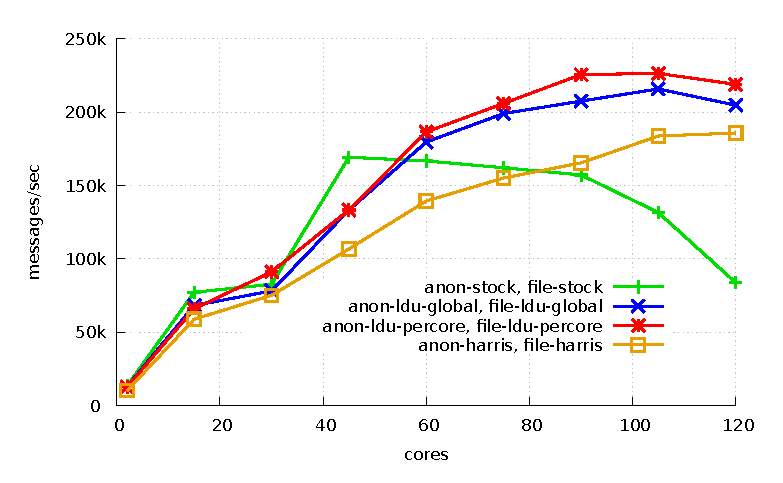
\includegraphics[scale=0.65]{graph/exim.eps}
  \end{center}
  \caption{Scalability of Exim. The stock Linux collapses after 60 core;in
  contrast, both unordered harris list and our \deferu flatten out.}
  \label{fig:exim}
\end{figure}
\subsection{Exim}
%$$$$$$$$$$$$$$$$$$$$$$$$$$$$$$$$$$$$$$$$$$$$$$$$$$$$$$$$$$$$$$$$$$$$$$$$$$$$$$$$
%Paragraph 1:  EXIM 실험 결과
%$$$$$$$$$$$$$$$$$$$$$$$$$$$$$$$$$$$$$$$$$$$$$$$$$$$$$$$$$$$$$$$$$$$$$$$$$$$$$$$$

\begin{figure}[tb]
  \begin{center}
    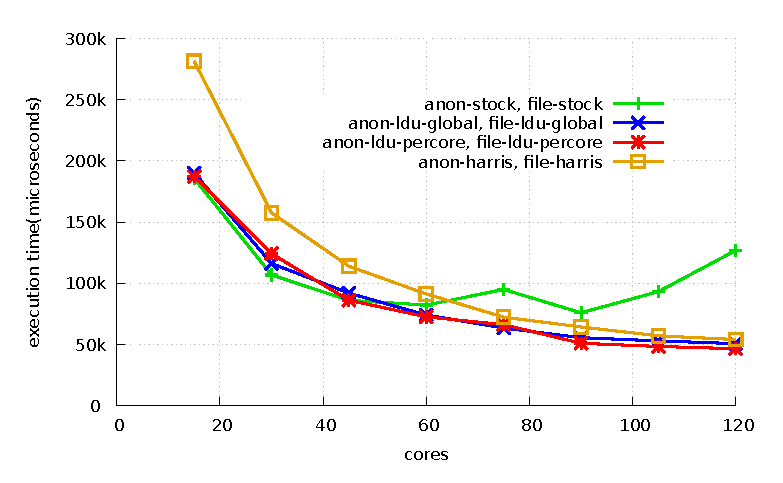
\includegraphics[scale=0.65]{graph/lmbench.eps}
  \end{center}
  \caption{Execution time of lmbench's fork micro benchmark. The fork micro
  benchmark drops down for all methods up to 15 core but either flattens out or
  goes up slightly after that. At 15 core, the stock Linux goes up;the others
  flattens out}
  \label{fig:MicroBench}
\end{figure}



%$$$$$$$$$$$$$$$$$$$$$$$$$$$$$$$$$$$$$$$$$$$$$$$$$$$$$$$$$$$$$$$$$$$$$$$$$$$$$$$$
%Paragraph 1: 워크로드에 대한 설명
%$$$$$$$$$$$$$$$$$$$$$$$$$$$$$$$$$$$$$$$$$$$$$$$$$$$$$$$$$$$$$$$$$$$$$$$$$$$$$$$$
To measure the performance of Exim, we used MOSBENCH, a many-core
scalability benchmark.
The Exim email server is designed to scale because the Exim delivers messages to
mail boxes in parallel using the Linux process;the Exim is a fork-intensive
workload.
clients run on the same machine and each client sends to a different user to
prevent contention on user mail file.
The Exim was bottlenecked by the filesystem since the message body appends to
the per-user mail file, so we used the separated tmpfs to reduce filesystem
bottleneck.

%$$$$$$$$$$$$$$$$$$$$$$$$$$$$$$$$$$$$$$$$$$$$$$$$$$$$$$$$$$$$$$$$$$$$$$$$$$$$$$$$
%Paragraph 2:실험 결과에 대한 설명
%$$$$$$$$$$$$$$$$$$$$$$$$$$$$$$$$$$$$$$$$$$$$$$$$$$$$$$$$$$$$$$$$$$$$$$$$$$$$$$$$
Results shown in Figure~\ref{fig:exim} show that Exim scales well up to 60 core
,but the stock Linux performance decreases near 60 core.
Both Harris and our LDU increase up to 105 core because they can execute
concurrent updates without semaphores.
These per-core queue performs better due to the fact that it reduce
cache coherence-related overheads outperforming stock Linux by 2.6x and Harris
by 1.2x.
Even though we applied the scalable solutions, the Exim shows the limitation
near 105 core since the Exim process has relatively large size of virtual
address mapping that leads to the clearing virtual address mappings overheads
and many soft page fault during the process destruction which execute more
slowly with more NUMA remote memory access.
The Harris has 15\% idle time, whereas per-core queue LDU
has 22\% idle time due to the LDU has the efficient algorithms.

\begin{figure*}[t!]
    \centering
    \begin{subfigure}[b]{0.33\textwidth}
        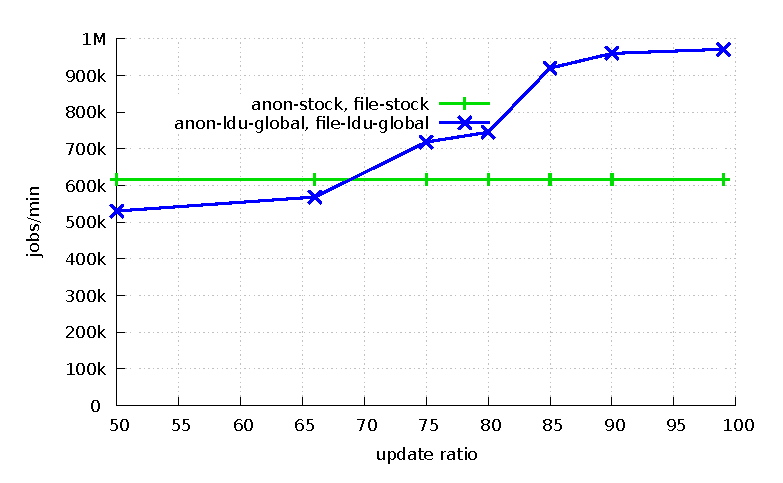
\includegraphics[height=1.3in]{graph/ratio_aim7.eps}
        \caption{AIM7 - 120core}
    \end{subfigure}%
    \begin{subfigure}[b]{0.33\textwidth}
        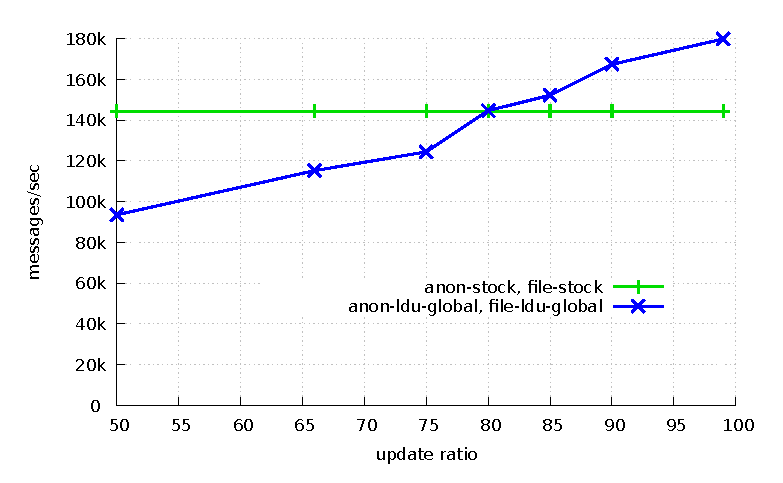
\includegraphics[height=1.3in]{graph/ratio_exim.eps}
        \caption{Exim - 120core}
    \end{subfigure}
    \begin{subfigure}[b]{0.33\textwidth}
        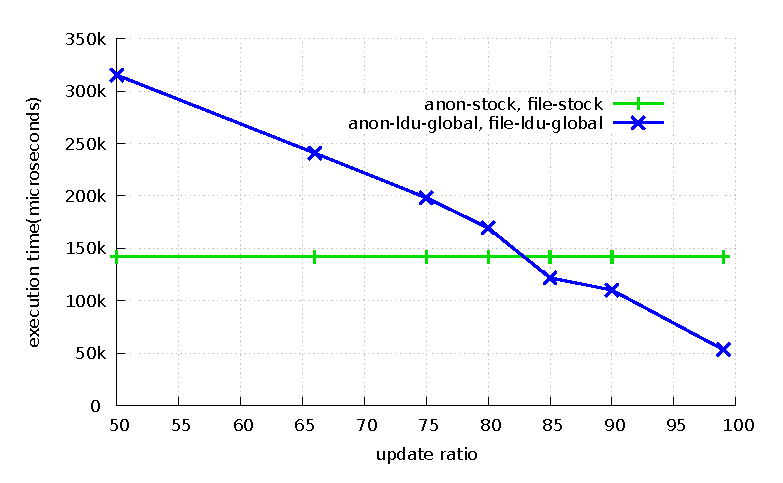
\includegraphics[height=1.3in]{graph/ratio_lmbench.eps}
        \caption{Lmbench - 120core}
    \end{subfigure}
        \centering
    \begin{subfigure}[b]{0.33\textwidth}
        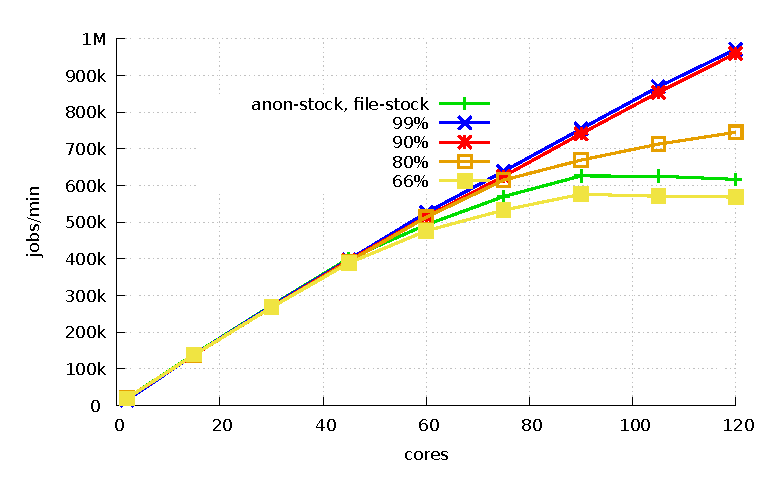
\includegraphics[height=1.3in]{graph/ratio_aim7_core.eps}
        \caption{AIM7 - scalability}
    \end{subfigure}%
    \begin{subfigure}[b]{0.33\textwidth}
        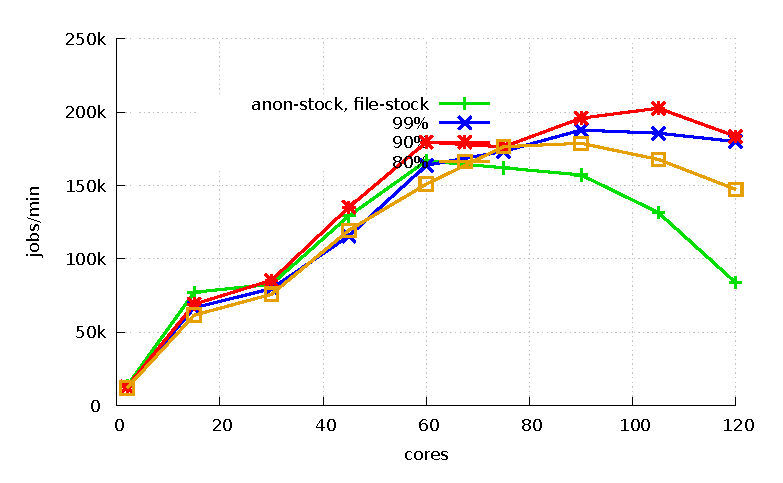
\includegraphics[height=1.3in]{graph/ratio_exim_core.eps}
        \caption{Exim - scalability}
    \end{subfigure}
    \begin{subfigure}[b]{0.33\textwidth}
        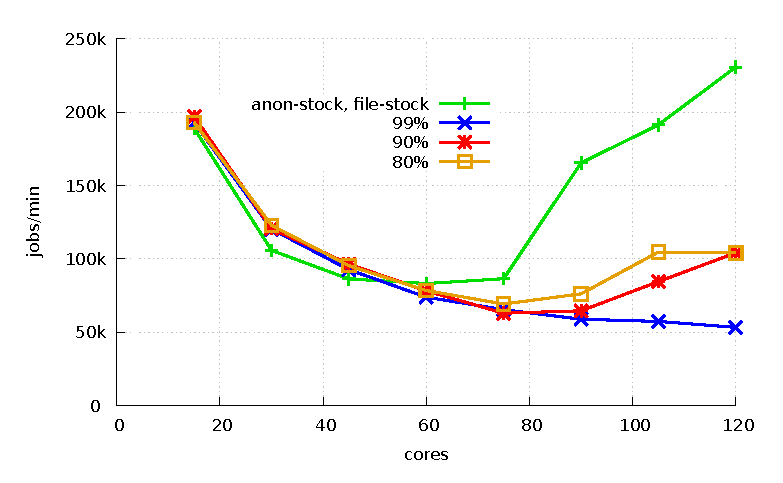
\includegraphics[height=1.3in]{graph/ratio_lmbench_core.eps}
        \caption{Lmbench - scalability}
    \end{subfigure}
    \caption{performance with read-write ratios on 120core and scalability with
    read-write ratios. the LDU can show substantial scalability where the data
    structures are frequently updates but rarely read. the scalability of AIM7
    shows that LDU substantially high scalability at the over the 90 percent
    update rate, and 80 percent update rates slightly.}
    
\end{figure*}

\subsection{Lmbench}
%$$$$$$$$$$$$$$$$$$$$$$$$$$$$$$$$$$$$$$$$$$$$$$$$$$$$$$$$$$$$$$$$$$$$$$$$$$$$$$$$
%Paragraph 1: %워크로드에 대한 설명
%$$$$$$$$$$$$$$$$$$$$$$$$$$$$$$$$$$$$$$$$$$$$$$$$$$$$$$$$$$$$$$$$$$$$$$$$$$$$$$$$
The Lmbench has various micro benchmarks including process management workloads.
We use executing the shell workload in the Lmbench.
This workload is used to measure the basic process primitives such as creating a
new process, running a program, and context switching.
We configured process create workload to enable the parallelism option(the
value is 1000).

%$$$$$$$$$$$$$$$$$$$$$$$$$$$$$$$$$$$$$$$$$$$$$$$$$$$$$$$$$$$$$$$$$$$$$$$$$$$$$$$$
%Paragraph 2: 실험 결과에 대한 설명
%$$$$$$$$$$$$$$$$$$$$$$$$$$$$$$$$$$$$$$$$$$$$$$$$$$$$$$$$$$$$$$$$$$$$$$$$$$$$$$$$
The results for the Lmbench are shown in Figure~\ref{fig:MicroBench}, 
and the results show the execution times.
Up to 45 core, the stock Linux scales linearly and then the execution time goes
up to grow.
The per-core LDU outperform stock Linux by 2.7x and and Harris by
1.1x at 120 core.
While stock Linux has 69\% idle time, other methods have approximately 35\%
idle time since stock Linux waits to acquire two rmap
semaphores(\code{anon\_vma's rwsem} and \code{mapping's i\_mmap\_rwsem}).

\subsection{Updates ratio}

%$$$$$$$$$$$$$$$$$$$$$$$$$$$$$$$$$$$$$$$$$$$$$$$$$$$$$$$$$$$$$$$$$$$$$$$$$$$$$$$$
%Paragraph 2:  실험을 수행한 이유
%$$$$$$$$$$$$$$$$$$$$$$$$$$$$$$$$$$$$$$$$$$$$$$$$$$$$$$$$$$$$$$$$$$$$$$$$$$$$$$$$
The LDU is a method for update-heavy data structure.
That is, the LDU can show substantial scalability where the data structures are
frequently updates but rarely read because the read operation executes the
synchronize function to apply logs.
That means the read operations can be slower.
Therefore, we wonder what acceptable LDU's update ratios for the update-heavy
data structure is.

To further evaluate LDU and to understand the effect of read operation, we
perform the additional read operation with respect to the rmap.
The anonymous rmap uses the version of ldu with global queue because we
merely focus on read ratio and then we sequentially increase read (lock and
synchronize) ratios regarding the file rmap.
The upper graphs of Figure x-x  shows the performance on 120 core depending
on read rate, and the lower graphs represent the scalability.

%$$$$$$$$$$$$$$$$$$$$$$$$$$$$$$$$$$$$$$$$$$$$$$$$$$$$$$$$$$$$$$$$$$$$$$$$$$$$$$$$
%Paragraph 2: 실험 결과에 대한 설명
%$$$$$$$$$$$$$$$$$$$$$$$$$$$$$$$$$$$$$$$$$$$$$$$$$$$$$$$$$$$$$$$$$$$$$$$$$$$$$$$$
Since the AIM7 has less fork-intensive workload feature than other ones, the
read operations are invoked relatively infrequently.
As a result, although the data structure uses 75\%(3
update, 1 read) update rate, the AIM7 has outstanding performance than stock
Linux.
The scalability of AIM7 shows that LDU substantially high scalability at the
over the 90\% update rate, and 80\% update rates slightly. 

%$$$$$$$$$$$$$$$$$$$$$$$$$$$$$$$$$$$$$$$$$$$$$$$$$$$$$$$$$$$$$$$$$$$$$$$$$$$$$$$$
%Paragraph 2: 실험 결과에 대한 설명
%$$$$$$$$$$$$$$$$$$$$$$$$$$$$$$$$$$$$$$$$$$$$$$$$$$$$$$$$$$$$$$$$$$$$$$$$$$$$$$$$
The result of the Exim and the Lmbench shows the more high fork-intensive
workload represents the read operations high effects

